% Chapter Template

\chapter{Experimental Results} % Main chapter title

\label{Chapter4} % Change X to a consecutive number; for referencing this chapter elsewhere, use \ref{ChapterX}

\lhead{Chapter 4. \emph{Experimental Results}} % Change X to a consecutive number; this is for the header on each page - perhaps a shortened title

%----------------------------------------------------------------------------------------
%	SECTION 1
%----------------------------------------------------------------------------------------

\section{Non-Combusting Tests}

In order to directly compare data between the different L/D ratios tested, it was important to keep the conditions nearly the same for all tests. For all non-combusting tests performed, the driver gas was helium at an initial pressure of 225 psi. The test gas was nitrogen at 0.5 psi and the expansion gas was helium at an initial pressure of 0.25 psi. This produced the freestream conditions as follows: M$_\infty$ = 2.32, U$_\infty$ = 2150 m/s, and T$_\infty$ of 411K. 

%-----------------------------------
%	SUBSECTION 2
%-----------------------------------
\subsection{Schlieren}

For each L/D, schlieren images were captured. Figures \ref{fig:5},\ref{fig:7}, and \ref{fig:9} show the effects the L/D ratio has on mixing abilities. It is clear that all of these cavities exhibit mixing and show signs of strong acoustic signals. The images captured for an L/D ratio of 5, however, show more disturbances, relatively, within the cavity itself. It is difficult to say with the images, though, how much more mixing exists within the cavity. Further sharpening of the images

Figure \ref{fig:5-30} shows the cavity with an angled downstream wall. With this image, it is very clear that there are little or no acoustic waves present. This is strong evidence in support of the angled wall's ability to suppress the oscillation acoustic waves. However, with the acoustic waves not present, it may be possible that the mixing within the cavity suffers as a result. This will be investigated with the combustion tests. 

Also captured by the schlieren imaging system is an indication of residence time within these cavities. Dust particles within the test section were dispersed in the flow and some of these particles were drawn into the cavity. Measuring how long these particles take to make one revolution within the cavity can provide an estimate of residence time. Figure \ref{fig:ResTime} shows one such particle traveling over several images. The particle took 68 frames to make one revolution, corresponding to an estimated residence time of about 850 $\mu$s. This corresponds well with the 1ms magnitude residence time achieved by Ben-Yakar \cite{ben2001cavity}.

%-----------------------------------
%    SUBSECTION 3
%-----------------------------------

\subsection{IR}

For some of these tests, IR emission data was captured to measure test time of the tests. The test times extracted from the IR data are displayed in Table \ref{Table:IRtest}. Of these test times, they all correspond to each other, which implies that conditions were reasonably the same for all tests. The theoretical test time, which was extracted from an X-T diagram, as shown in Figure \ref{fig:XT}, was about 559 $\mu$s for theses tests. However, the compressible flow equations used in generating these X-T diagrams assume the flow to be inviscid. However, due to viscous effects that are present in the tube, the experimental test time will be less than the theoretical test time, which is consistent with the data.

\begin{table}[]
\centering
\caption[Test time calculated with IR signal]{Test time from IR signal. M$_\infty$=2.34, Theoretical test time = 559$\mu$s.}
\label{Table:IRtest}
\begin{tabular}{c|c}

Test Number & Test Time ($\mu$s) \\ \hline
046         & 399                      \\ 
048         & 443                      \\ 
049         & 441                      \\ 
050         & 424                      \\ 
\end{tabular}
\end{table}

Each test produced an IR trace similar to the one shown in Figure\ref{fig:IRtrace}. As can be seen in this trace, the slit width was too wide for the test, so the IR sensor captured some light scattered forward, as indicated by the sloped increase in voltage signal. The signal also includes a lower "shelf" signal. This level is currently thought to be the light produced by burning diaphragm particles traveling down the tube. Regardless, the test gas is indicated by the highest level of the signal. Test time is taken to be the time between points halfway between the lowest and highest value of the test signal. With this method, a consistent measure of test time can be achieved regardless of the amount of forward scattering of light. 


%----------------------------------------------------------------------------------------
%	FIGURES
%----------------------------------------------------------------------------------------
\newpage

\begin{figure}
\centering
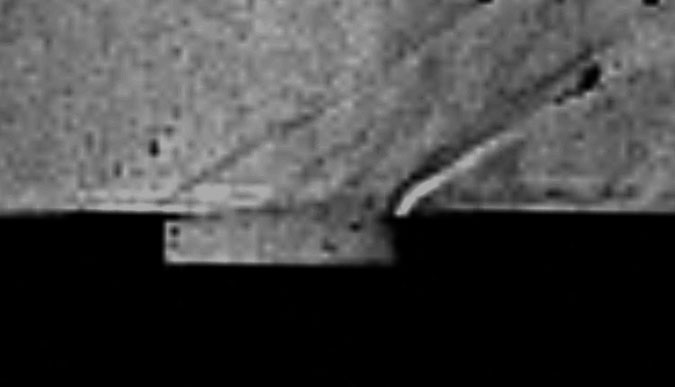
\includegraphics[height = 3in]{Figures/5.jpg}
\caption[Schlieren image of cavity. L/D = 5.]{Schlieren image of cavity. L/D = 5.}
\label{fig:5}
\end{figure}

\begin{figure}
\centering
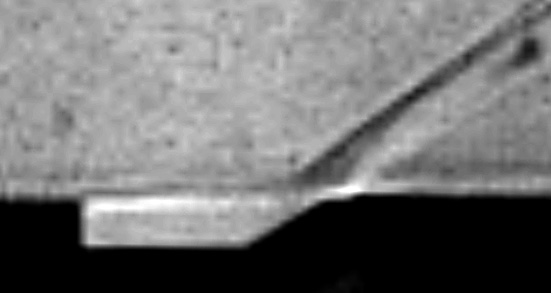
\includegraphics[height = 3in]{Figures/5-30.jpg}
\caption[Schlieren image of cavity with angled downstream wall. L/D = 5.]{Schlieren image of cavity. L/D = 5. Downstream wall angle = 30$^\circ$}
\label{fig:5-30}
\end{figure}

\begin{figure}
\centering
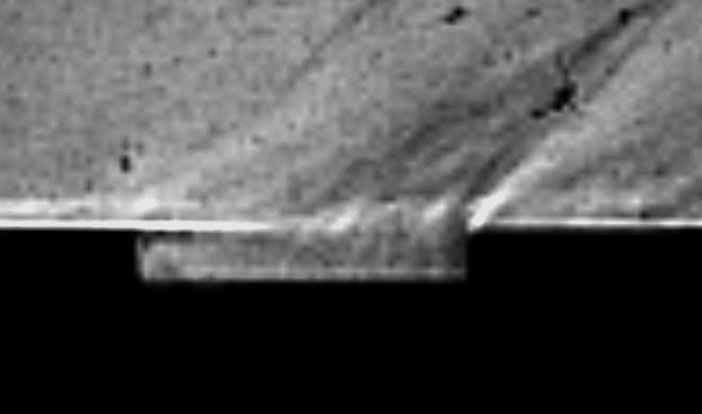
\includegraphics[height = 3in]{Figures/7.jpg}
\caption[Schlieren image of cavity. L/D = 7.]{Schlieren image of cavity. L/D = 7.}
\label{fig:7}
\end{figure}

\begin{figure}
\centering
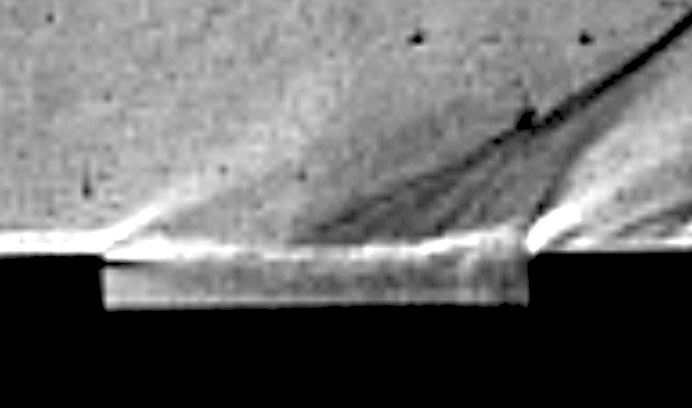
\includegraphics[height = 3in]{Figures/9.jpg}
\caption[Schlieren image of cavity. L/D = 9.]{Schlieren image of cavity. L/D = 9.}
\label{fig:9}
\end{figure}

\begin{figure}[p!]
\centering
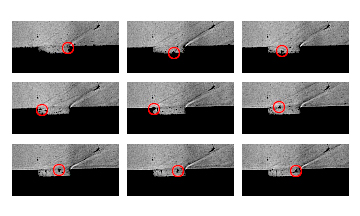
\includegraphics[width = \textwidth]{Figures/cavResTime.jpg}
\caption[Time-correlated Schlieren image of cavity. L/D = 5.]{Time-correlated Schlieren image of cavity. L/D = 5. 9 frames out of 68 are shown. Residence time = 850 $\mu$s.}
\label{fig:9}
\end{figure}
\clearpage

\begin{figure}
\centering
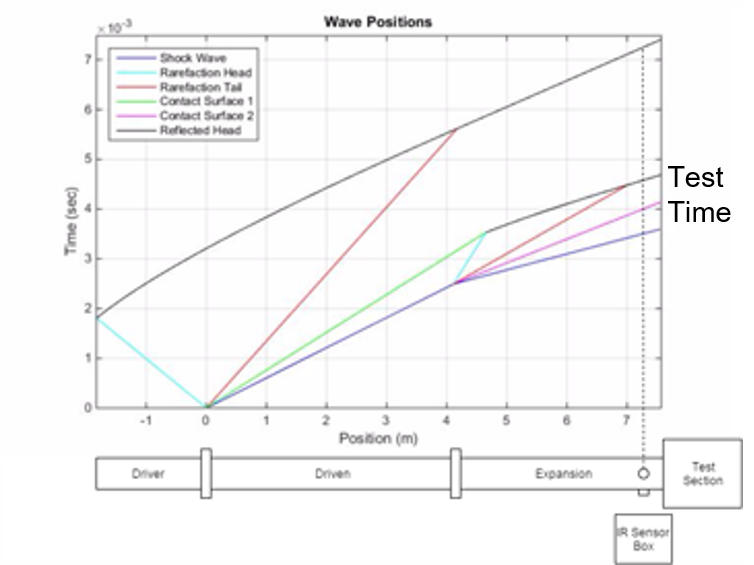
\includegraphics[height = 3in]{Figures/XTDiag.png}
\caption[X-T Diagram of Cavity Tests]{X-T diagram generated from the initial conditions of the cavity tests: P4 = 225psi, P1=0.5psi, P$_e$=0.25psi. The test gas was nitrogen.}
\label{fig:XT}
\end{figure}

\begin{figure}
\centering
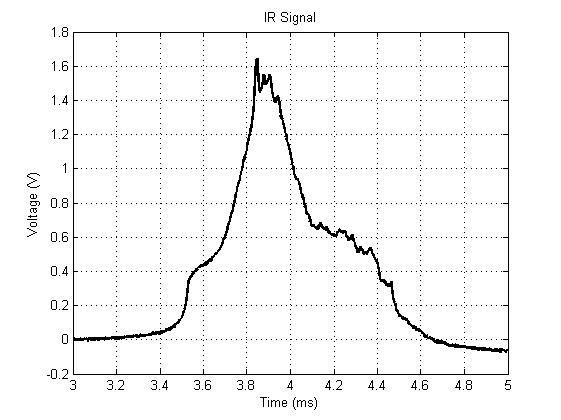
\includegraphics[height = 3in]{Figures/Emission.jpg}
\caption[IR Signal for Test 046]{IR Signal for Test 046. P4 = 225psi, P1=0.5psi, P$_e$=0.25psi. The test gas was a 95\% Nitrogen and 5\% CO$_2$ mixture. Test Time = 399 $\mu$s.}
\label{fig:IRTrace}
\end{figure}

